%-----------------------------------LICENSE------------------------------------%
%   This file is part of Mathematics-and-Physics.                              %
%                                                                              %
%   Mathematics-and-Physics is free software: you can redistribute it and/or   %
%   modify it under the terms of the GNU General Public License as             %
%   published by the Free Software Foundation, either version 3 of the         %
%   License, or (at your option) any later version.                            %
%                                                                              %
%   Mathematics-and-Physics is distributed in the hope that it will be useful, %
%   but WITHOUT ANY WARRANTY; without even the implied warranty of             %
%   MERCHANTABILITY or FITNESS FOR A PARTICULAR PURPOSE.  See the              %
%   GNU General Public License for more details.                               %
%                                                                              %
%   You should have received a copy of the GNU General Public License along    %
%   with Mathematics-and-Physics.  If not, see <https://www.gnu.org/licenses/>.%
%------------------------------------------------------------------------------%
%   Author:     Ryan Maguire                                                   %
%   Date:       June 24, 2025                                                  %
%------------------------------------------------------------------------------%
\documentclass{beamer}
\usepackage{graphicx}
\usepackage{amsmath}
\usepackage{tikz}
\usetikzlibrary{decorations.markings, arrows.meta}
\graphicspath{{../images/}}
\title{Knots, Groups, and Quandles}
\author{Ryan Maguire}
\date{July 15, 2025}
\usenavigationsymbolstemplate{}
\setbeamertemplate{footline}[frame number]
\begin{document}
    \maketitle
    \begin{frame}{Outline}
        \begin{itemize}
            \item Combinatorial representations of knots.
            \item Groups and quandles.
            \item How to handle groups and quandles using a computer.
        \end{itemize}
    \end{frame}
    \begin{frame}{Combinatorial Representations of Knots}
        The common invariants of knot theory are very hard to compute, even
        with a computer. But still, it is easier for a computer to do these
        things, hence we need to get the knot into the computer.
        \par\hfill\par
        There are several ways to do this:
        \begin{enumerate}
            \item
                Gauss code.
            \item
                Planar Diagram (PD) code.
            \item
                Dowker-Thistlethwaite (DT) code.
            \item
                Many more.
        \end{enumerate}
    \end{frame}
    \begin{frame}{Combinatorial Representations of Knots}
        Given a knot diagram with $N$ crossings, Gauss code is a string with $3N$,
        PD code is a string that is $4N$ long, and DT code is $N$ characters long.
        Each has its benefits. Extended Gauss code can distinguish mirrors,
        DT code cannot.
        PD code is perhaps the easiest to
        reconstruct the knot diagram, and DT code is the shortest.
        \par\hfill\par
        To obtain the DT code of
        a knot diagram, place your finger on the knot and \textit{walk} along
        the diagram, labelling the crossings. When you get back to your starting
        point each crossing will have two numbers associated with it. It is
        not difficult to see that each crossing will have exactly one odd number
        and one even number. For each even number, if that number was associated
        with an \textit{over} crossing (that is, your finger ran over the
        crossing as you were labelling it), place a minus sign in front. Write
        out the pairs of integers as $(0,a_{0})$, $(2,a_{1})$, $\dots$,
        $(2n-2,a_{n-1})$. The DT code is the list $a_{0},a_{1},\dots,a_{n-1}$.
    \end{frame}
    \begin{frame}{Combinatorial Representations of Knots}
        Try it out.
        \begin{figure}
            \centering
            \resizebox{!}{0.75\textheight}{%
                \includegraphics{trefoil_knot_oriented_with_labels}
            }
            \caption{Oriented Trefoil with Crossings Labeled.}
        \end{figure}
    \end{frame}
    \begin{frame}{Combinatorial Representations of Knots}
        If we stick to knots with no more than 26 crossings, we can replace
        numbers with letters. We use lowercase for numbers with a $+$ sign, and
        uppercase for numbers with a $-$ sign. The trefoil becomes
        \texttt{bca}.
    \end{frame}
    \begin{frame}{Combinatorial Representations of Knots}
        Planar Diagram code (PD code) is handled as follows. We again start at
        some arbitrary point, walk along the knot, and label the \textit{arcs}.
        At each under crossing we write down the arcs, starting with the one
        behind us (the one our fingers were coming from),
        and going around the crossing clockwise.
        \par\hfill\par
        We write \texttt{X[a, b, c, d]}, where each letter represents one of the
        four arcs. PD code is the sequence of $N$ such labels, one for each
        under crossing.
    \end{frame}
    \begin{frame}{Combinatorial Representations of Knots}
        Try it out.
        \begin{figure}
            \centering
            \resizebox{!}{0.75\textheight}{%
                \includegraphics{trefoil_knot_arcs_labeled}
            }
            \caption{Oriented Trefoil with Arcs Labeled}
        \end{figure}
    \end{frame}
    \begin{frame}{Combinatorial Representations of Knots}
        For the trefoil, we get:
        \begin{equation}
            \texttt{X[1, 4, 2, 5]},\,
            \texttt{X[3, 0, 4, 1]},\,
            \texttt{X[5, 2, 0, 3]}
        \end{equation}
        If $K$ is a knot diagram with $N$ crossings, then for any label
        \texttt{X[a, b, c, d]}, we have $c-a=1\operatorname{mod}N$.
        Why?
        \par\hfill\par
        What is $d-b$? What does this number tell us?
    \end{frame}
    \begin{frame}{Combinatorial Representations of Knots}
        PD code is one of the most common means of representing knots into a
        computer. It can distinguish mirrors, and two prime knots have the same PD
        code if and only if they are equivalent.
        \par\hfill\par
        DT code is shorter, and some knot theorists (such as those who work in
        tabulation) often do not differentiate between a knot and its mirror,
        nor do they differentiate between a knot and its \textit{inverse}.
        Because of this, many data sets will list out knots using DT code.
    \end{frame}
    \begin{frame}{Groups and Quandles}
        You now know roughly how to get a knot into a computer. Later we will
        talk about using Jupyter notebooks, together with some Python code, and
        have a computer do some real calculations.
        \par\hfill\par
        For now, let's consider the following question. Suppose you have a group
        or a rack or a quandle, and you know it has finitely many elements.
        How can you represent it into a computer?
    \end{frame}
    \begin{frame}{Groups and Quandles}
        A group is a set $G$ with a binary operation $*$ that satisfies:
        \begin{enumerate}
            \item
                $a*(b*c)=(a*b)*c$ (Associativity).
            \item
                There is some $e\in{G}$ with $e*a=a*e=a$ for all $a\in{G}$
                (Identity).
            \item
                For each $a\in{G}$ there is an $a^{-1}\in{G}$ such that
                $a*a^{-1}=e$ (Inverses).
        \end{enumerate}
    \end{frame}
    \begin{frame}{Groups and Quandles}
        For finite groups you can start with some \textit{generating set} and
        create a \textit{graph} for the group by connecting elements of the group
        using these generators. This is called a \textit{Cayley Graph}.
    \end{frame}
    \begin{frame}{Groups and Quandles}
        \begin{figure}
            \centering
            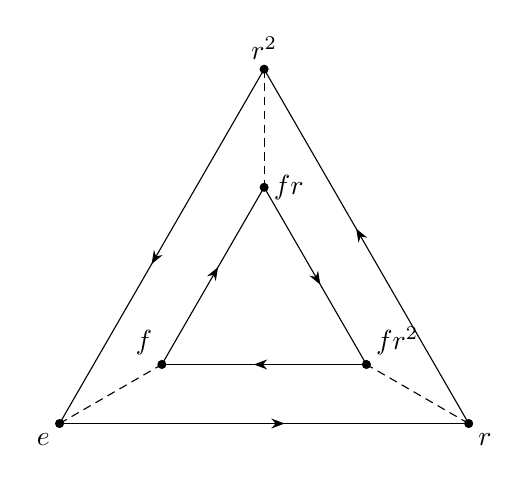
\begin{tikzpicture}[%
                ->-/.style = {%
                    decoration = {%
                        markings,
                        mark = at position 0.55 with \arrow{Stealth}
                    },
                    postaction = {decorate}
                }
            ]

                % The coordinates for the outer triangle.
                \coordinate (e) at (210.0:3.0);
                \coordinate (r) at (330.0:3.0);
                \coordinate (r2) at (90.00:3.0);

                % The coordinates for the inner triangle.
                \coordinate (f) at (210.0:1.5);
                \coordinate (fr2) at (330.0:1.5);
                \coordinate (fr) at (90.00:1.5);

                % Dots for the coordinates.
                \foreach\x in {e, r, r2, f, fr, fr2}{%
                    \draw[fill = black] (\x) circle (0.05);
                }

                % Solid arrows for rotations.
                \draw[->-] (e) to (r);
                \draw[->-] (r) to (r2);
                \draw[->-] (r2) to (e);
                \draw[->-] (f) to (fr);
                \draw[->-] (fr) to (fr2);
                \draw[->-] (fr2) to (f);

                % Dashed arrows for reflections.
                \draw[densely dashed] (e) to (f);
                \draw[densely dashed] (r) to (fr2);
                \draw[densely dashed] (r2) to (fr);

                % Label the nodes.
                \node at (e) [below left] {$e$};
                \node at (r) [below right] {$r$};
                \node at (r2) [above] {$r^{2}$};
                \node at (f) [above left] {$f$};
                \node at (fr) [right] {$fr$};
                \node at (fr2) [above right] {$fr^{2}$};
            \end{tikzpicture}
        \end{figure}
    \end{frame}
    \begin{frame}{Groups and Quandles}
        Groups have a lot of structure. In particular, they have the (right)
        \textit{Latin square property}: For each
        $a,b\in{G}$ there is a unique $x\in{G}$ such that $a*x=b$. That is,
        in a group we can solve linear equations. Do quandles have this property?
        \par\hfill\par
        A quandle is a set $Q$ with a binary operation $*$ such that:
        \begin{enumerate}
            \item
                $a*a=a$.
            \item
                For each $a,b\in{Q}$, there is an $x\in{Q}$ such that
                $a*x=b$.
            \item
                $a*(b*c)=(a*b)*(a*c)$.
        \end{enumerate}
        So yes, quandles have the (right) Latin square property. Because of this,
        you might try to use graphs to represent quandles, but this is rarely done.
    \end{frame}
    \begin{frame}{Groups and Quandles}
        Graphs are certainly objects that can be easily represented into a
        computer, so perhaps our job is done. But there are other methods that
        we should explore as well.
        \par\hfill\par
        A \textit{free group} on $n$ letters is the set of all finite combinations
        of these letters and there \textit{inverses}, up to simplification, and
        with the operation of concatenation.
        \par\hfill\par
        For example, if $n=2$, we can take the letters to be $a$, $b$.
        $ab$ is one such element of the free group, as is $aba$, $aab$,
        $abab$, $a^{-1}ba$, and so on. The only simplification we allow is for
        $a$ to cancel $a^{-1}$ and $b$ to cancel $b^{-1}$,
        \textbf{provided they are adjacent}.
    \end{frame}
    \begin{frame}{Groups and Quandles}
        \begin{figure}
            \centering
            \resizebox{!}{0.75\textheight}{%
                \includegraphics{cayley_graph_free_group}
            }
            \caption{Cayley graph for $F(a,\,b)$.}
        \end{figure}
    \end{frame}
    \begin{frame}{Groups and Quandles}
        A \textit{presentation} of a group is a \textit{quotient} of a
        free group, subject to some \textit{relations}.
        For example, the integers $\mathbb{Z}$ can be thought of as the
        free group on one letter, $\mathbb{Z}=F(a)$. The group of
        two elements, $\mathbb{Z}_{2}$, is then the quotient of $F(a)$ with
        the relation $a^{2}=e$. We would write:
        \begin{equation}
            \mathbb{Z}_{2}\equiv
            \langle{a}\;|\;a^{2}=e\rangle
        \end{equation}
        Some authors would simply write $a^{2}$ instead of $a^{2}=e$.
    \end{frame}
    \begin{frame}{Groups and Quandles}
        How can we represent the trivial group?
    \end{frame}
    \begin{frame}{Groups and Quandles}
        Question: Given two groups, with two different presentations,
        is it possible to tell them apart?
    \end{frame}
    \begin{frame}{Groups and Quandles}
        Question: Given a presentation for a group $G$, is it possible to
        tell if $G$ has more than 1 element?
    \end{frame}
    \begin{frame}{Groups and Quandles}
        Sometimes yes, sometimes no. Here are a few common groups from topology:
        \begin{align}
            \langle{a,\,b}\;|\;ab=ba\rangle
            &=
            \mathbb{Z}^{2}\\
            \langle{a,\,b}\;|\;aba=b\rangle
            &=
            \mathbb{Z}\rtimes\mathbb{Z}_{2}
        \end{align}
        We can tell that these ones are not trivial with a little bit of effort.
        In general, it is impossible to determine if a given group is trivial
        from just a presentation. This is called the \textbf{word problem}.
    \end{frame}
    \begin{frame}{Groups and Quandles}
        The \textit{fundamental group} of a space is the set of all
        \textit{loops} (like loops of string), modulo \textit{homotopy}, and the
        group operation is concatenation of loops. The \textbf{knot group} of
        a knot $K\subseteq\mathbb{R}^{3}$ is the fundamental group of the knot
        complement $\mathbb{R}^{3}\setminus{K}$.
        \par\hfill\par
        There is something called the Wirtinger presentation for this group,
        and it is very special in that the word problem for these types of groups
        is indeed decideable. You can in principle have a computer check whether
        or not two knot groups are the same.
    \end{frame}
    \begin{frame}{Groups and Quandles}
        There are similar notions for quandles (presentation, relations,
        free quandles, etc.), and in particular there is an invariant called the
        \textit{fundamental quandle} of a knot. Quite interestingly, this is a
        near perfect invariant (it does not distinguish mirrors or inverses),
        and the word problem for it is decideable. So you might think, alas,
        knot theory is solved! We're done!
        \par\hfill\par
        In principle, sure, but in practice this problem is far to hard to work
        with. I know of no attempt to implement these algorithms in a real computer.
    \end{frame}
    \begin{frame}{How to Handle Groups and Quandles Using a Computer}
        The simplest way of working with groups and quandles in a computer is via
        the \textbf{Cayley table}. Given a group or quandle with $N$ elements,
        we create an $N\times{N}$ grid where the $(n,\,m)$ slot is the product
        $a_{n}*a_{m}$, where $a_{n}$ is the $n^{\textrm{th}}$ element and
        $a_{m}$ is the $m^{\textrm{th}}$ element.
    \end{frame}
    \begin{frame}{How to Handle Groups and Quandles Using a Computer}
        Here is a simple example.
        \begin{table}
            \centering
            \begin{tabular}{c|cc}
                +&0&1\\
                \hline
                0&0&1\\
                1&1&0
            \end{tabular}
            \caption{Cayley Table for $\mathbb{Z}_{2}$}
        \end{table}
    \end{frame}
    \begin{frame}{How to Handle Groups and Quandles Using a Computer}
        Several questions arise instantle. How many Cayley tables are there
        for groups of size $N\times{N}$? How many for quandles?
        Can we train a machine learning algorithm to detect if a random
        grid of numbers is a Cayley table for a group? For a quandle?
    \end{frame}
    \begin{frame}{How to Handle Groups and Quandles Using a Computer}
        In our next class we will talk more about cocycles and some more
        computational things involving racks and quandles.
    \end{frame}
\end{document}
